\subsection{Aufbau}
\begin{figure}[h]
  \centering
  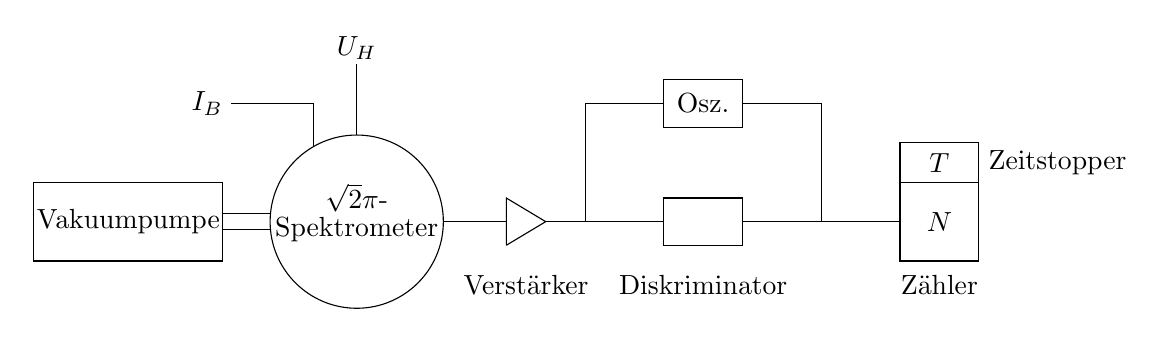
\begin{tikzpicture}
    \draw (0,0) rectangle (2.4,1);
    \draw (1.2,0.5) node {Vakuumpumpe};
    \draw (2.4,0.4)--(3,0.4);
    \draw (2.4,0.6)--(3,0.6);
    \draw (4.1,0.5) circle (1.1);
    \draw (4.1,0.8) node {$\sqrt{2}\pi$-};
    \draw (4.1,0.4) node {Spektrometer};
    \draw (5.2,0.5)--(6,0.5);
    \draw (6,0.2)--(6,0.8)--(6.5,0.5)--(6,0.2);
    \draw (6.25,-0.3) node {Verstärker};
    \draw (6.5,0.5)--(8,0.5);
    \draw (8,0.2) rectangle (9,0.8);
    \draw (8.5,-0.3) node {Diskriminator};
    \draw (9,0.5)--(11,0.5);
    \draw (11,0) rectangle (12,1);
    \draw (11.5,-0.3) node {Zähler};
    \draw (11.5,0.5) node {$N$};
    \draw (11,1) rectangle (12,1.5);
    \draw (11.5,1.25) node {$T$};
    \draw (13,1.25) node {Zeitstopper};
    \draw (7,0.5)--(7,2)--(8,2);
    \draw (10,0.5)--(10,2)--(9,2);
    \draw (8,1.7) rectangle (9,2.3);
    \draw (8.5,2) node {Osz.};
    \draw (3.55,1.453)--(3.55,2)--(2.5,2);
    \draw (2.2,2) node {$I_B$};
    \draw (4.1,1.6)--(4.1,2.5);
    \draw (4.1,2.7) node {$U_H$};
  \end{tikzpicture}
  \caption{schematische Skizze des Versuchsaufbaus}
  \label{fig:aufbau}
\end{figure}

Der Versuchsaufbau ist in Abbildung \ref{fig:aufbau} zu sehen. Das $\sqrt{2}\pi$-Spektrometer wird mit einer Vakuumpumpe evakuiert, damit die Elektronen und Positronen frei fliegen können. Der Strom der das Magnetfeld erzeugt kann an einem Drehregler eingestellt werden. Über eine Hallsonde kann die entsprechende Hallspannung $U_H$ gemesen und an einer Anzeige abgelesen werden. An dem Spektroskop kann außerdem über eine Art Blende der Transmissionsgrad eingestellt werden. Je kleiner der Transmissionsgrad, desto genauer muss der Eintreffwinkel der Teilchen im Spektrometer sein. Das analoge Signal des Detektors im Spektrometer wird verstärkt und anschließend wandelt ein Diskriminator die Signale ab einer bestimmten Schwellenspannung in eine logische EINS um. Für die Einstellung der Schwellenspannung kann das Signal vor und nach dem Diskriminator auf einem Oszilloskop beobachtet werden. Die logischen Signale werden anschließend während eines einstellbaren Zeitfensters $T$ gezählt und angezeigt.

\subsection{Messung zur Bestimmung des Offsets von $U_H$}
Zunächst wird die Offsetspannung der Hallsonde bestimmt, damit der um diesen Offset korrigierte Wert proportional zum Magnetfeld ist. Um den Offset zu bestimmen kann die Hysteresekurve ausgenutzt werden. Dazu wird die komplette Hysteresekurve über die Variation von $I_B$ fünf mal durchlaufen. Für jeden Durchgang werden die Hallspannungen $U_\pm$ bei $I_B=0$ notiert. Ohne Offset würde aufgrund der Symmetrie der Hysteresekurve $U_++U_-=0$ gelten. Durch den Offset $\delta U$ gilt aber $U_++U_-=2\delta U$. \\

\subsection{Kalibrationsmessung}
Damit ein Zusammenhang zwischen $U_H$ und den jeweiligen Teilchenimpulsen bestimmt werden kann wird das Emissionsspektrum von Barium ($^{137}$Ba) aufgenommen. Dazu wird zunächst die Diskriminatorschwelle so eingestellt, dass der Untergrund nur einen kleinen Teil des Signales ausmacht, aber trotzdem vernünftige Zählraten im zweistelligen Bereich (bei $T=\SI{40}{\second}$) zustande kommen. Der Untergrund wird bei falschherum (für Barium) gepoltem Magnetfeld für \SI{200}{\second} aufgenommen. Anschließend wird der positive Bereich von $U_H$ in Schritten von 10 Skalenteilen (SKT) durchlaufen und jeweils für \SI{40}{\second} gezählt (bei 1\% Transmission). In dem Spektrum sind zwei Konversionslinien zu erkennen. Diese werden noch einmal genauer in Schritten von 0,5 SKT vermessen. In einer Feinmessung wird der Bereich der Konversionslinien noch bei 1\% Transmission aufgenommen. Dabei wird die Hallspannung in Schritten von  0,5 SKT variiert und jeweils für \SI{100}{\second} gezählt.

\subsection{Vermessung von Natrium und Thallium}
Für Natrium ($^{22}$Na) und Thallium ($^{204}$Tl) wird das gesammte Spektrum in Schritten von etwa 7 SKT vermessen. Es wird bei 4\% Transmission und für 40 Sekunden gemessen. Da für die Messungen der Diskriminator neu eingestellt wird, wird auch die Untergrundmessung wiederholt. Es ist darauf zu achten, dass $^{22}$Na im Gegensatz zu den beiden anderen Stoffen ein $\beta^+$-Strahler ist, also das Magnetfeld umgepolt werden muss.
